\clearpage

\section{TI Amplifier}

\maketitle

This block has one input signal and one output signal both corresponding to electrical signals. The output signal corresponds to the amplification of the input signal with added noise.


\subsection*{Input Parameters}

\begin{itemize}
	\item amplification\{1e6\}
	\item noiseamp\{ 1e-4 \}
\end{itemize}

\subsection*{Methods}
 
TIAmplifier() {}
\bigbreak
TIAmplifier(vector$<$Signal *$>$ \&InputSig, vector$<$Signal *$>$ \&OutputSig) :Block(InputSig, OutputSig) {}
\bigbreak
void initialize(void)
\bigbreak
bool runBlock(void)
\bigbreak
void setAmpplification(\texttt{t\_real} Amplification)
\bigbreak
void setNoiseAmpplitude(\texttt{t\_real} NoiseAmplitude)

\subsection*{Functional description}

The output signal is the product of the input signal with the parameter \textit{amplification} plus a component that corresponds to the noise introduced by the amplification of the signal. 

\pagebreak

\subsection*{Input Signals}

\subparagraph*{Number:} 1

\subparagraph*{Type:} Electrical (TimeContinuousAmplitudeContinuousReal)

\subsection*{Output Signals}

\subparagraph*{Number:} 1

\subparagraph*{Type:} Electrical (TimeContinuousAmplitudeContinuousReal)

\subsection*{Examples} 

\begin{figure}[h]
	\centering
	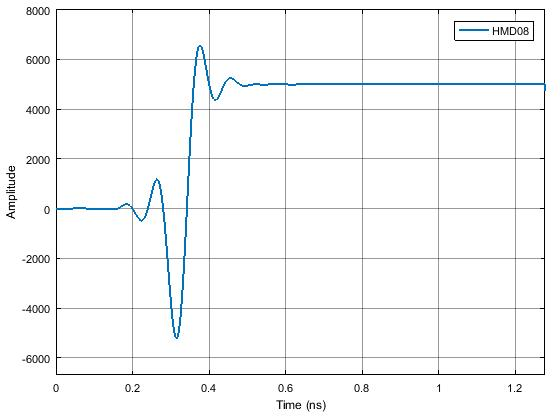
\includegraphics[width=\textwidth]{../homodyne_receiver/figures/TIAmplifier_output}
	\caption{Example of the output signal of the amplifier block for a binary sequence 01. Note the scale of the y axis in comparison to the one in the output signal of the photodiode. The shape of the signal is the same as expected}\label{TIAmplifier_output}
\end{figure}

\subsection*{Sugestions for future improvement}

